\documentclass[11pt,titlepage]{article}
\usepackage{geometry}
\geometry{
	a4paper,
	left=20mm,
	right=20mm,
	top=15mm,
	bottom=15mm,
}
\usepackage{tikz}
\usetikzlibrary{arrows,backgrounds}
\usepgflibrary{shapes.multipart}
\usepackage{graphicx}
\usepackage{mathtools}
\usepackage{inputenc}
\usepackage{amssymb}
\usepackage{wrapfig}
\usepackage{seqsplit}
\usepackage{float}
\usepackage[font=scriptsize]{caption} 
\linespread{1.0}
\usepackage{caption}
\renewcommand{\figurename}{Fig.}
\usepackage{subcaption}
\usepackage[title]{appendix}
\usepackage{enumitem}
\usepackage{listings}
\usepackage{xcolor}
\definecolor{codegreen}{rgb}{0,0.6,0}
\definecolor{codegray}{rgb}{0.5,0.5,0.5}
\definecolor{codepurple}{rgb}{0.58,0,0.82}
\definecolor{backcolour}{rgb}{0.95,0.95,0.92}

\lstdefinestyle{mystyle}{
	backgroundcolor=\color{backcolour},   
	commentstyle=\color{codegreen},
	keywordstyle=\color{magenta},
	numberstyle=\tiny\color{codegray},
	stringstyle=\color{codepurple},
	basicstyle=\ttfamily\tiny,
	breakatwhitespace=false,         
	breaklines=true,                 
	captionpos=b,                    
	keepspaces=true,                 
	numbers=left,                    
	numbersep=5pt,                  
	showspaces=false,                
	showstringspaces=false,
	showtabs=false,                  
	tabsize=2
}

\lstset{style=mystyle}
\setlength{\columnsep}{5pt}

%opening
\title{EECE6036: Intelligent Systems\\Homework \# 4}
\author{Zuguang Liu (M10291593)}



\begin{document}

\maketitle

\section{Denoising Autoencoder}





\subsection{Problem Statement}

An autoencoder shall be implemented by a two-layer neural network to remove noise applied to the MNIST dataset. Then the performance and the model itself is compared with the autoencoder constructed in Homework \#3, whose purpose was simply to reconstruct the images. 

To tell apart the two models, from now on the report uses \textbf{denoising autoencoder} to address this new network, and call the previous one \textbf{reconstructing autoencoder}.









\subsection{System Description}
Using the same stratified sampling policy the previous Homework used, the preprocessing section partitions the total 5,000 data points into 4,000 for training and 1,000 for testing, where there are 400 and 100 images for each model respectively. Over the training, each image is tempered with noise by a certain policy as input, and the original image is learned as target to fulfill the denoising purpose. 

\textbf{The noise policy generates ``salt and pepper'' noise} (salt pixels = 1, pepper pixels = 0) whose densities are approximately 5.56\% and 44.44\%. This is due to the fact that the dark ($<$ 0.5) vs bright pixels ($>$ 0.5) in an image is at a ratio around 8:1 on average, and the goal of total noise density = 50\%. 

The autoencoder is implemented by a 2-layer neural network with a hidden layer and an output layer. \textbf{The hidden layer incorporates 128 neurons} that transfer the noisy image into a 128-dimensional feature space. Then the output layer brings the reduced feature space back into the original 784 pixel values but with reduced noise. \textbf{Both layers use the \textit{sigmoid} activation function} (\ref{eqn:sigmoid}) \textbf{and a weight initialization scheme known as ``Xavier initialization''} showed in (\ref{eqn:xavier}), where $\mathcal{U}[a,b]$ is the uniform distribution within the interval between $a$ and $b$, $n_{in}$ is the input dimension of a layer, and $n_{out}$ is the output dimension of a layer \cite{glorot_understanding_nodate}.

\begin{equation}
	f(x) = \frac{1}{1+e^{-x}}, \  f'(x) = f(1-f)
	\label{eqn:sigmoid}
\end{equation}

\begin{equation}
	W \sim \mathcal{U} \bigg[  -\sqrt{\frac{6}{n_{in}+n_{out}}} , \  \sqrt{\frac{6}{n_{in}+n_{out}}} \ \bigg]
	\label{eqn:xavier}
\end{equation}

The training of the model is done by back propagation per data point, repeated for multiple epochs. 1,000 data points are separated for validation, presented to the model every 10 epochs, resulting in a series of on-line training errors. Within one epoch, the remaining 3,000 points are shuffled, then used to adjust weights and biases. The error is calculated with the average $J_2$ loss over all data points in the validation set, shown in (\ref{eqn:j2}), where $N$ is the number of data points, $y_i^n$ and $\hat{y}_i^n$ are the original and predicted $i$-th pixel value on the $n$-th image, respectively. 
\begin{equation}
	\bar{J_2} = \frac{1}{N} \sum_{n=1}^{N} J_2 = \frac{1}{1000} \sum_{n=1}^{1000} \bigg( \frac{1}{2} \sum_{i=1}^{784} (y_i^n - \hat{y}_i^n)^2 \bigg)
	\label{eqn:j2}
\end{equation}

To further improve the training, several mechanisms are used in the training algorithm, including:
\begin{enumerate}[label=\alph*.]
	\item Using \textbf{Weight decay} for regularization by adding a weight penalty term to the loss function, as in (\ref{eqn:weight_decay}) where $\boldsymbol{\lambda = 10^{-4}}$.
	\begin{equation}
		J = \bar{J_2} + \lambda \sum_{Layers L} \  \sum_{j \in Layer L} \  \sum_{i \in Layer L+1} \ w_{ij}^2
		\label{eqn:weight_decay}
	\end{equation}

	\item The gradient decent has an additional term to implement \textbf{momentum}, demonstrated in (\ref{eqn:bp_moment}), where \textbf{$\boldsymbol{\eta = 0.05$, $\alpha = 0.8}$}. 

	\begin{equation}
		\Delta w_{ij}(t) = -\eta \frac{\partial J}{\partial w_{ij}} + \alpha \Delta w_{ij} (t-1)
		\label{eqn:bp_moment}
	\end{equation}
	
%	\item \textbf{Operating thresholds of 0.25 and 0.75} are used so that output $\in [0, 0.25)$ is considered 0 when the corresponding truth is 0, and output $\in (0.75, 1]$ is considered 1 when the corresponding truth is 1. 
	
	\item Though the total repetition is 500 epochs, \textbf{an early stopping policy} is used so that it stops when the on-line training loss \textbf{does not improve more than $\boldsymbol{10^{-3}}$ for 50 epochs} compared to the minimum loss over the whole training session. As the validation set used for on-line testing is separate from the data used in back propagation, this ensures the model does not overfit the data. 
\end{enumerate}

After training, the resulting model is analyzed by feeding in the test dataset. A reconstructing autoencoder with the same hyper-parameters and policies except zero noise is also trained and tested for comparison.












\subsection{Results}
For the sake of discussion, both autoencoders are included in plots. Though the prediction is compared against the original image for both models, the reconstructing autoencoder has the exact same image as input, but the denoising autoencoder has noisy images as input. 
\subsection{Overall Performance}
Fig. \ref{fig:autoenc_test} demonstrates the performance of the autoencoders overall and on each class, where the error is calculated by (\ref{eqn:j2}). The on-line training error vs epochs is shown in Fig. \ref{fig:autoenc_train}. 

\begin{figure}[H]
	\centering
	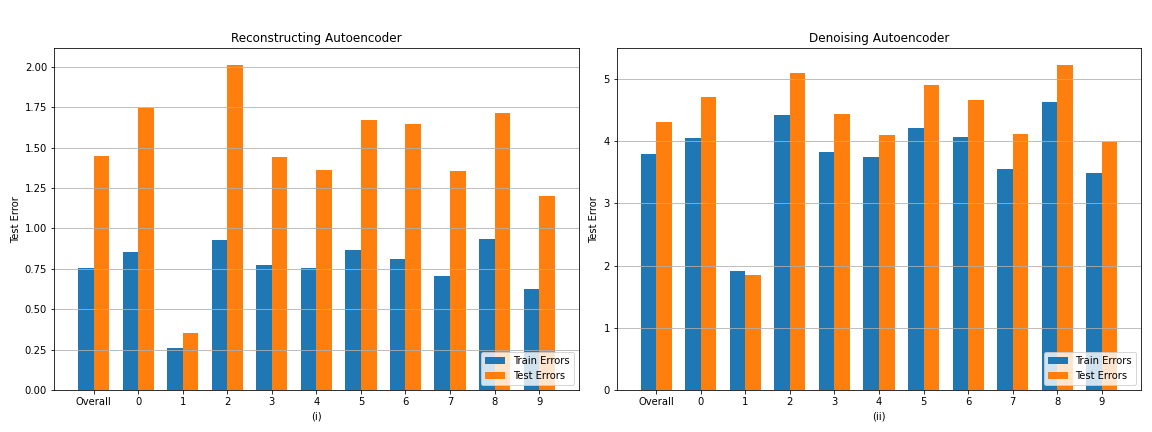
\includegraphics[width=\linewidth]{img/h4p1_test}
	\caption{Performance of the autoencoders on the training and test set}
	\label{fig:autoenc_test}
\end{figure}

\begin{figure}[H]
	\centering
	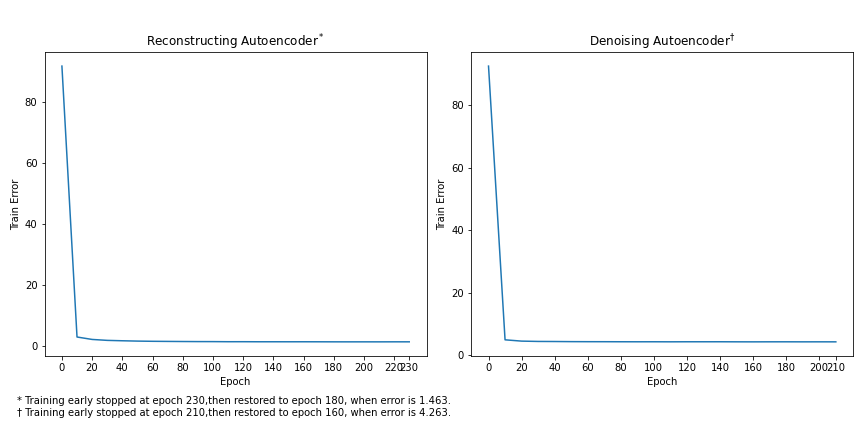
\includegraphics[width=\linewidth]{img/h4p1_train}
	\caption{On-line training error vs training epochs over time}
	\label{fig:autoenc_train}
\end{figure}








\subsection{Features}

Weights of 20 neurons in the hidden layer of the two networks are illustrated by 28 $\times$ 28 images in Fig. \ref{fig:autoenc_feature}, as the feature space is 784-dimensional, in accordance to 784 pixels of the original images. Though neurons are chosen randomly, the selection of neurons in both model uses the same indexes, so that neurons in the same position are compared.

\begin{figure}[H]
		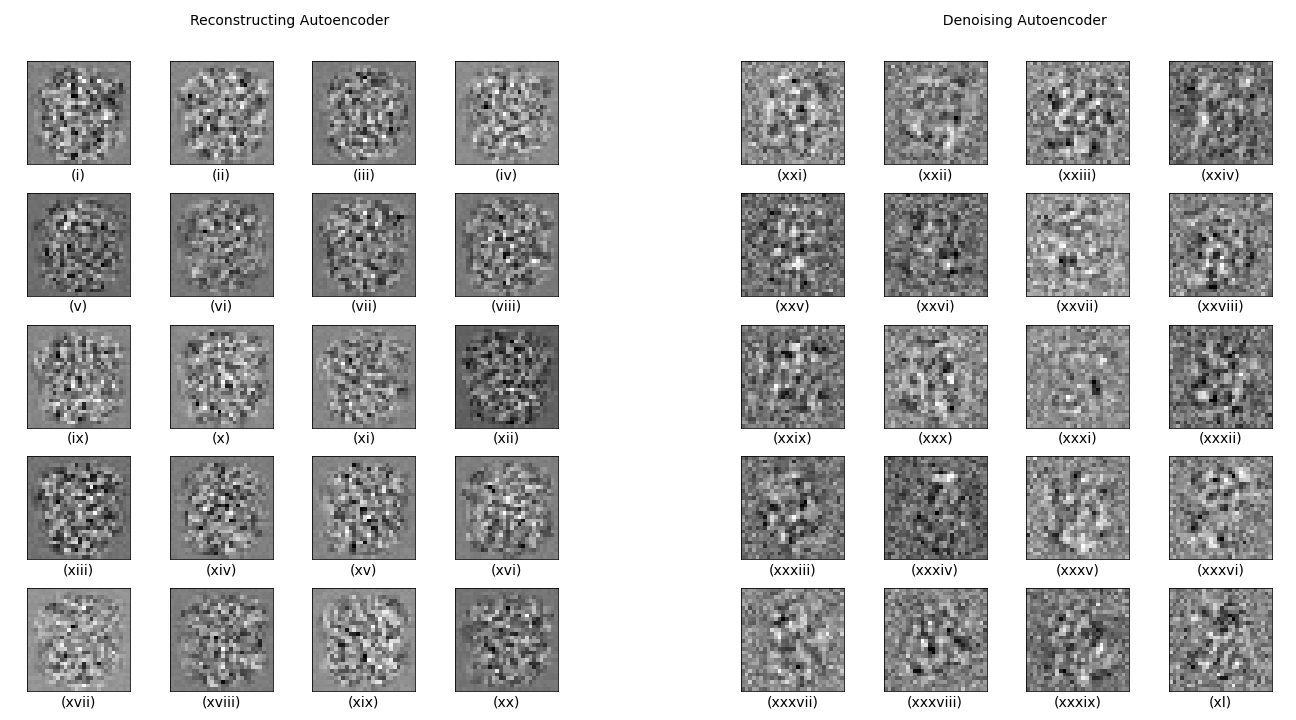
\includegraphics[width=\linewidth]{img/h4p1_feature}
		\caption{Feature map of 20 neurons in the hidden layer of both autoencoders.}
		\label{fig:autoenc_feature}
\end{figure}








\subsection{Sample Outputs}

Fig. \ref{fig:autoenc_output} uses 8 sets of images to visualize the two model's performance in reconstruction and noise removal.

\begin{figure}[htb]
	\centering
	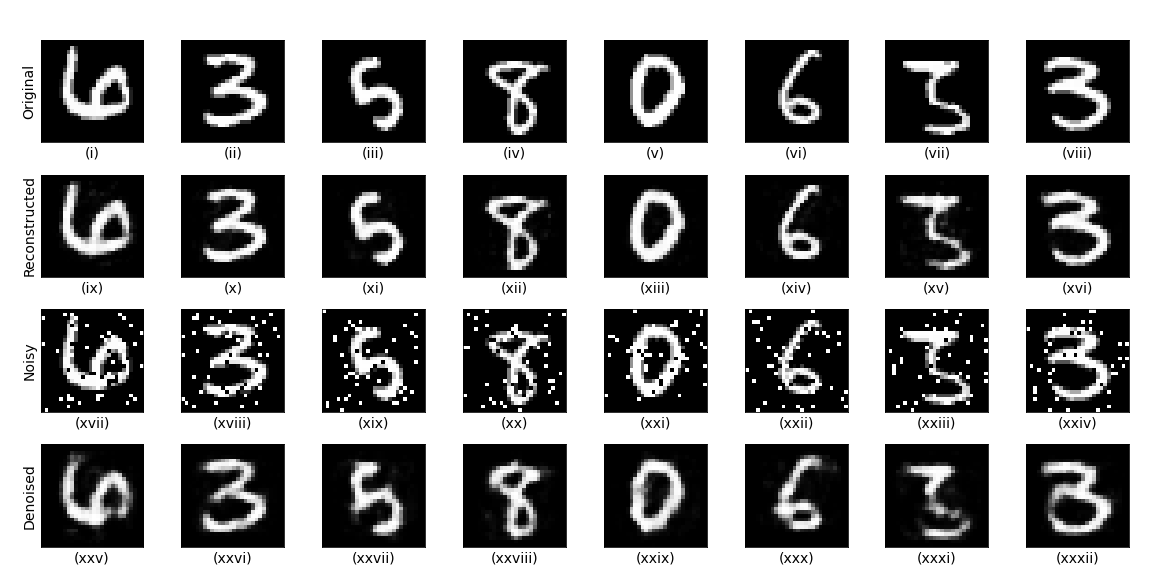
\includegraphics[width=\linewidth]{img/h4p1_outputs}
	\caption{Sample output of the models, (ix) - (xvi) for the reconstructing autoencoder, and (ix) - (xvi) for the denoising autoencoder}
	\label{fig:autoenc_output}
\end{figure}


\newpage
\subsection{Analysis of Results}
Observed from Fig. \ref{fig:autoenc_output}, both autoencoders serve their respective purposes well. Comparing the denoised images in with the original images, the ``salt and pepper'' noise is significantly reduced with minor errors. It is found that images with noise more scattered such as (xxiii) are denoised better than those with clustered noise such as (xxvii), due to the fact that clustered ``salt'' or ``pepper'' could be recognized as original pattern to remain.

Comparing the feature maps in their hidden layers, first difference to notice is that there are granular difference in each pixels throughout in the denoising autoencoder, which is absent in the reconstructing autoencoder. Moreover, larger clouds of dark or light pixels are in denoising autoencoder compared to the reconstructing one. It is theorized that the two differences could imply the denoising model learned a ``bigger picture'' in the image compared to reconstructing model, despite having larger training and testing error shown in Fig. \ref{fig:autoenc_test} and \ref{fig:autoenc_train}.

\newpage
\section{Classifiers Based on Autoencoders}
\subsection{Problem Statement}

Using the first layer from the autoencoders, two classifiers are constructed with an output layer that predicts the label of images instead. After training, the performance of the two networks shall be compared and contrasted together with the classifier from Homework \#3 whose hidden layer is initialized randomly.

To tell apart the models, the report uses \textbf{denoising classifier} to address the model based on denoising autoencoder, and calls the reconstruction-based network \textbf{reconstructing classifier}. The other one from Homework \#3 whose hidden layer is initialized randomly shall be called \textbf{BP classifier} as the gradient back-propagates to the first layer to adjust its weights, while only the output layer applies the weight change for the other two models.







\subsection{System Description}
To control the training settings, \textbf{all three classifiers} (reconstructing, denoising and BP) \textbf{are trained with exactly the same algorithm and hyper-parameters. }

As the problem states, \textbf{the two classifiers use a hidden layer with 128 neurons} from the denoising and reconstructing autoencoder, and an output layer that classifies images with an array of 10 elements, each of which represents the probability that the image can belong to a class. \textbf{This output layer is again implemented by sigmoid (\ref{eqn:sigmoid}) and Xavier initialization policy (\ref{eqn:xavier}).} 

The training of the models proceeds similarly to that of the autoencoders, except the prediction is compared against the labels of the images rather than the image itself. Original version of the images is used as input for both models, since it could be unfair for the reconstructing and BP classifer. There are other minor modifications in the training session, including:

\begin{enumerate}
	\item The back propagation uses momentum-based gradient descent (\ref{eqn:bp_moment}) with 
	$\boldsymbol{\eta = 0.01, \alpha = 0.8}$ and weight decay uses $\boldsymbol{\lambda = 10^{-5}}$.
	\item Only weights of the output layer change over training. The hidden layer is treated as ``read-only''.
	\item The loss is calculated by (1 - balanced accuracy), where the balanced accuracy is the hit rate when comparing the true class and the predicted class using ``winner-take-all'' strategy over the output array.
	\item \textbf{Operating thresholds of 0.25 and 0.75 are used} so that output $\in [0, 0.25)$ is considered 0 when the corresponding truth is 0, and output $\in (0.75, 1]$ is considered 1 when the corresponding truth is 1. 
	\item Early stop strategy is again used for regularization. \textbf{The training stops when no improvement is observed for 50 epochs. }
\end{enumerate}

After training, test dataset is presented to all models including reconstructing classier, denoising classifier and BP classifier.








\subsection{Results}
Time series of on-line training loss on both models is presented in Fig. \ref{fig:classifier_train}. Fig. \ref{fig:classifier_cm} shows the confusion matrices of both classifiers on train data and test data, along with the ones of BP classifier. 

\begin{figure}[H]
	\centering
	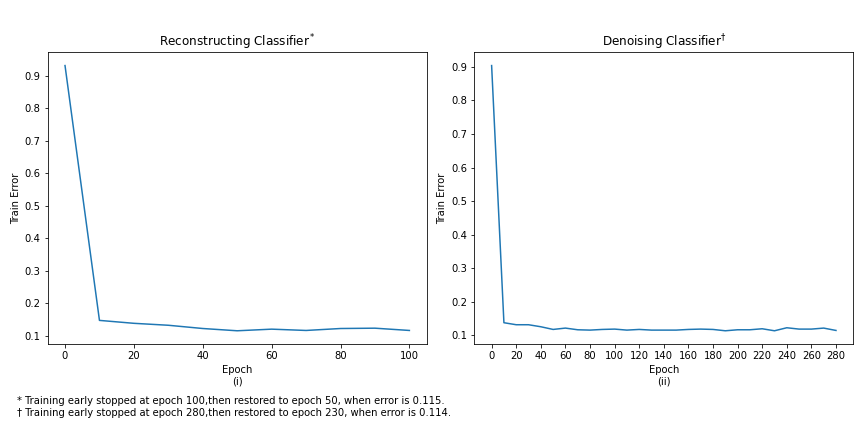
\includegraphics[width=\linewidth]{img/h4p2_train}
	\caption{Error vs epochs during training of reconstructing classifier, denoising classifier and BP classifier}
	\label{fig:classifier_train}
\end{figure}

\begin{figure}[H]
	\centering
	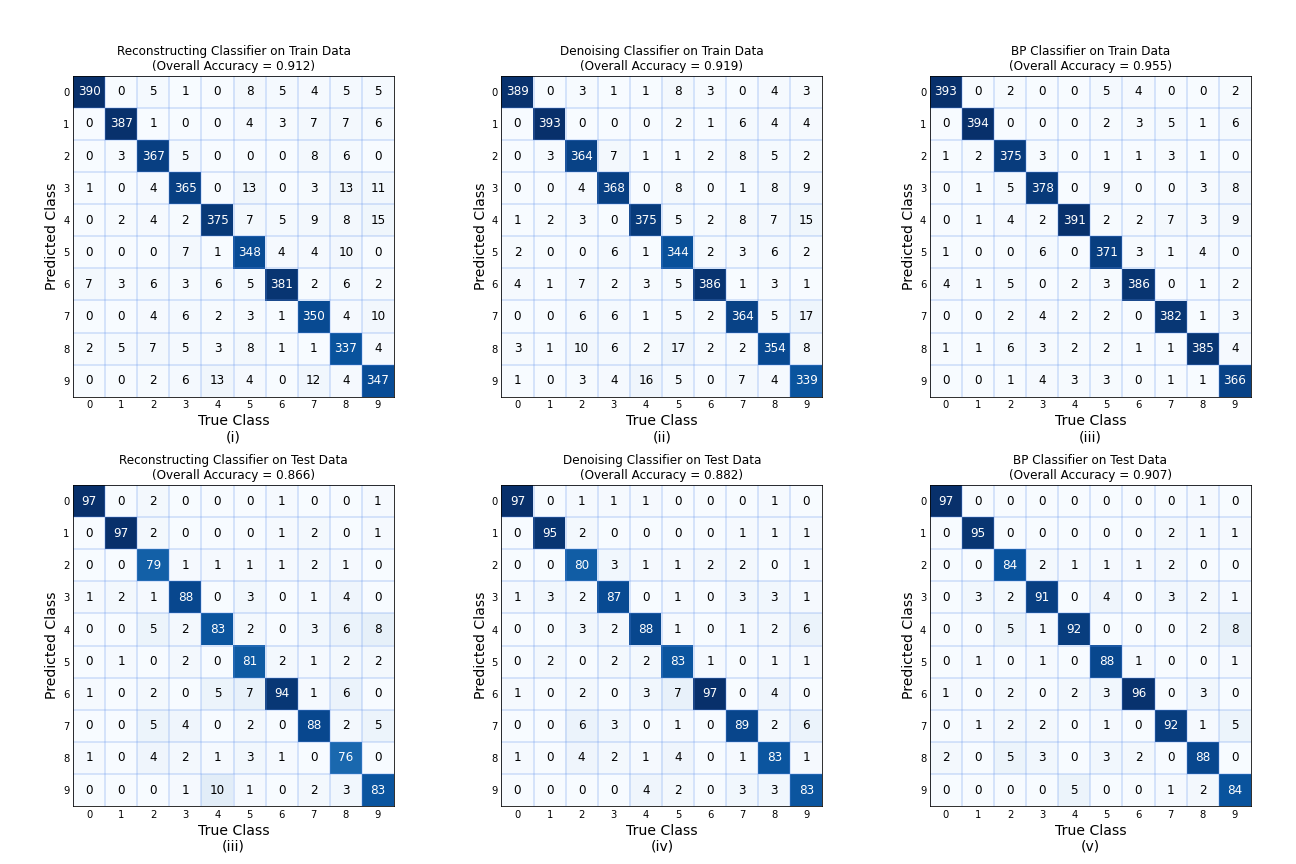
\includegraphics[width=\linewidth]{img/h4p2_cm}
	\caption{Performance of reconstructing classifier, denoising classifier and BP classifier}
	\label{fig:classifier_cm}
\end{figure}

\newpage
\subsection{Analysis of Results}
Unfortunately, neither the reconstructing nor the denoising classifier beat the BP classifier in performance (Fig. \ref{fig:classifier_cm}). If to rank their accuracy in classifying, BP is better than denoising, and the  reconstructing one is the worst. To break down the analysis, I will discuss the difference between each other separately. 

The fact that reconstructing classifier performs worse than the denoising classifier on all classes is not surprising. As the hypothesis in Section 1.4 states, the denoising autoencoder generalizes the image more than the reconstructing autoencoder, and thus, each perceptron in the hidden layer is less likely to be restricted to a small amount of pixels. Comparatively, perceptrons in the reconstructing autoencoder are more likely to miss the global information, which could be important in classification problems.

The denoising classifier has the potential to perform better than the BP classifier, since the train error experienced an amount of up-and-down's in Fig. \ref{fig:classifier_train} (ii). Yet it did not manage to win in the end. This could be caused by the fact that it only has 10 neurons to train, while the BP classifier has 138 (128 in layer 1, 10 in layer 2). The pre-trained well-performing autoencoder layer may have established a good basis for the feature reduction, but the inability to fine tune the hidden 128 neurons makes it hard to achieve high-resolution training no matter how long the training lasts. If the pre-trained autoencoder weights are used as a weight initialization policy rather than a ``read-only'' layer, it is believe that the model could have even better performance and training efficiency than the BP classifier.







\vfill
\bibliography{refs}
\bibliographystyle{ieeetr}

\newpage
\begin{appendices}
\section{Python Code: preprocess.py}
\lstinputlisting[language=Python]{code/preprocess.py}

\newpage
\section{Python Code: nn.py}
\lstinputlisting[language=Python]{code/nn.py}

\newpage
\section{Python Code: p1\_train.py}
\lstinputlisting[language=Python]{code/h4p1_train.py}

\newpage
\section{Python Code: p1\_test.py}
\lstinputlisting[language=Python]{code/h4p1_test.py}

\newpage
\section{Python Code: p2\_train.py}
\lstinputlisting[language=Python]{code/h4p2_train.py}

\newpage
\section{Python Code: p2\_test.py}
\lstinputlisting[language=Python]{code/h4p2_test.py}

\end{appendices}

\end{document}